\chapter{Models}
\label{sec:models}
Our algorithm will generate an emulation using vertex disjoint subgraph homeomorphism. For this purpose, we will use vertex-multilabeled directed simple graphs as defined in Definition \ref{def:graph}. In this model, we chose to use a single vertex for a unit that can be either a lut or a logic cell instead of different vertices for each. This is because for our ECP5 use case, we only encounter such logical units with `flexible' functionality. In these graphs we will:

\begin{itemize}
\item ..model a wire as a vertex that may be connected with any number of vertices in either direction of types ``$\mathit{arc}$", any number of incoming edges from ``$\mathit{port\_out}$" vertices and any number of outgoing edges to ``$\mathit{port\_in}$" edges.
\item ..model a transistor as a vertex with a label ``$\mathit{arc}$" and a label ``$\mathit{configurable}$" for configurable transistors or label ``$\mathit{unconfigurable}$" for unconfigurable transistors (that are not counted towards label compatibility). It has an incoming edge from the source ``$\mathit{wire}$" of the transistor and an outgoing edge to the target ``$\mathit{wire}$" of the transistor.
\item ..model a logical unit with LUT- and register functionality as a vertex with label $``\mathit{slice}"$ that only has connections from vertices with label ``$\mathit{port\_in}$" and to vertices with label ``$\mathit{port\_out}$".
\item ..model an input of a logical unit as a vertex with label ``$\mathit{port\_in}$" and an outgoing directed edge towards a ``$\mathit{slice}$" vertex and an incoming edge from a ``$\mathit{wire}$" vertex.
\item ..model an output of a logical unit as a vertex with label ``$\mathit{port\_out}$" and an incoming directed edge from a ``$\mathit{slice}$" vertex and an outgoing edge to a ``$\mathit{wire}$" vertex.
\end{itemize}

An example of such am model is shown in Figure \ref{fig:graphmodel-logiccell} where a graph model is shown of the logic cell in Figure \ref{fig:logiccell}.

\begin{figure}
\centering
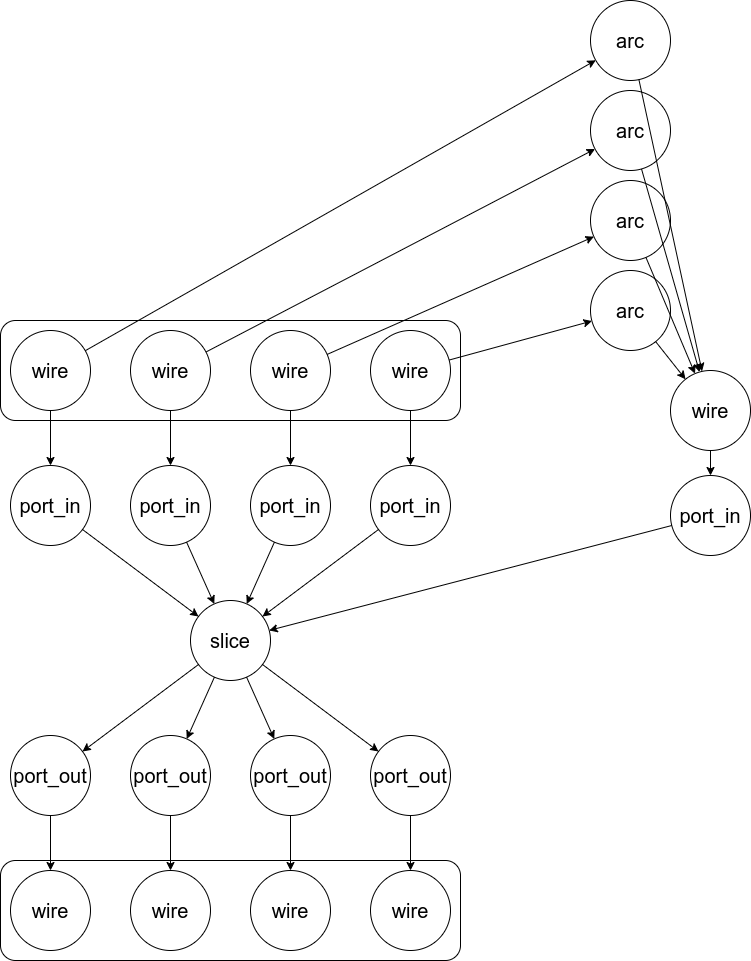
\includegraphics[width=0.5\textwidth]{images/modelOfCell.png}
\caption{Graph model of the logic cell shown in Figure \ref{fig:logiccell}}
\label{fig:graphmodel-logiccell}
\end{figure}
